\documentclass[tikz]{standalone}

\colorlet{FilledSurface}{blue!20}
\colorlet{FilledSurfaceGroupOne}{blue!20}
\colorlet{FilledSurfaceGroupTwo}{red!20}
\colorlet{FilledSurfaceGroupThree}{green!20}
\colorlet{FilledSurfaceGroupFour}{magenta!20}
\colorlet{FormulaBackground}{green!10}
\colorlet{FormulaFrame}{green}


\begin{document}
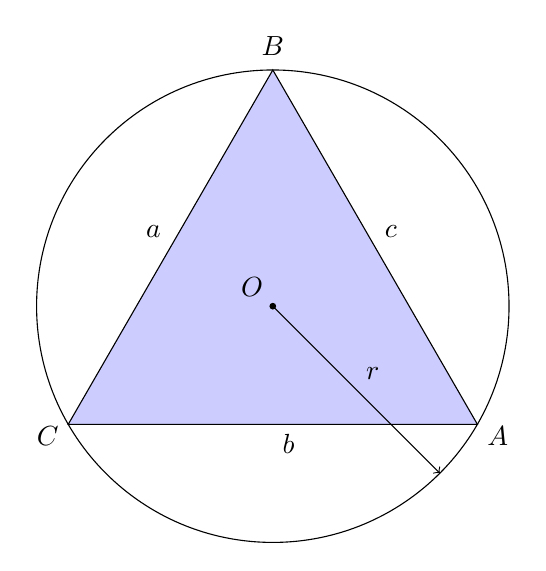
\begin{tikzpicture}

    \def\circumradius{3}
    \def\angleA{330}
    \def\angleB{90}
    \def\angleC{210}

    \coordinate (center) at (0, 0);
    \draw (center) circle (\circumradius);
    \coordinate (A) at (\angleA:\circumradius);
    \coordinate (B) at (\angleB:\circumradius);
    \coordinate (C) at (\angleC:\circumradius);
    \draw[fill=FilledSurfaceGroupOne]
    (A) -- node [above right] {$c$}
    (B) -- node [above left] {$a$}
    (C) -- node [below right] {$b$}
    cycle;

    \def\offset{0.3}
    \node at (\angleA:\circumradius+\offset) {$A$};
    \node at (\angleB:\circumradius+\offset) {$B$};
    \node at (\angleC:\circumradius+\offset) {$C$};

    \draw[fill=black] (center) circle (1pt) node [above left] {$O$};
    \draw[->] (center) -- node [above right] {$r$} (315:\circumradius);

\end{tikzpicture}
\end{document}

% \myPolygonArea{ABC} = \dfrac{abc}{4R}
